\section{Shape formation}
\begin{frame}
\only<1-2>{
	\frametitle{Shape formation}
	\only<1>{
		\textbf{Objective:} Distributed algorithm to generate a desired shape \cite{MR-AC-RN:2014}. 
	}
	\begin{columns}
		\begin{column}{0.5\textwidth}
			\begin{itemize}
				\only<1>{
					\item \textbf{Guides:} Index $0,1,2$ acts as reference for coordinate axis by continuously transmitting their index.
				}
				\only<2>{
					\item \textbf{Builders:} Index $3$ onwards for shape formation
					\item For forming a linear shape of width 2, the \textbf{shape matrix} would look like
					\vspace{0.2cm}
					\begin{align*}
					\label{eq:shape_matrix_linear}
					\begin{bmatrix}
					&Index & N_1 & DD_1 & N_2 & DD_2 &\\ 
					\cline{2-6}\\
					&3      & 1      & 1      & 2      & 1        &\\
					&4      & 2      & 1      & 3      & \sqrt{2} & \\
					&5      & 3      & 1      & 4      & 1        &\\
					&\cdots & \cdots & \cdots & \cdots & \cdots   &
					\end{bmatrix}
					\end{align*}
					\newline
					where,\\
					$N_i:$ Desired neigbour i\\ $DD_i$: Desired distance from neighbour i.
				}
			\end{itemize}
		\end{column}
		\begin{column}{0.5\textwidth}
			\only<1>{
				\begin{figure}
					\centering
					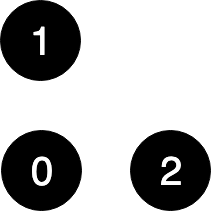
\includegraphics[scale=0.25]{shape_formation_process_guides}
				\end{figure}
			}
			\only<2->{
				\begin{figure}
					\centering
					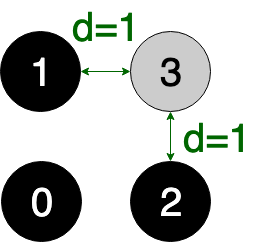
\includegraphics[scale=0.25]{shape_formation_sm_1}
					\hspace{0.9cm}
				\end{figure}
			}
			\only<2->{
				\begin{figure}
					\centering
					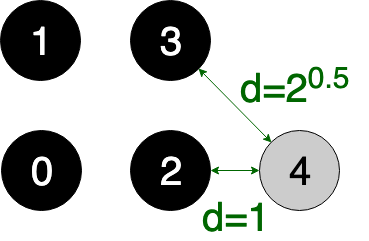
\includegraphics[scale=0.25]{shape_formation_sm_2}
				\end{figure}
			}
		\end{column}
	\end{columns}
}
\only<3>{
	\frametitle{\small Flowchart}
	\begin{figure}
		\centering
		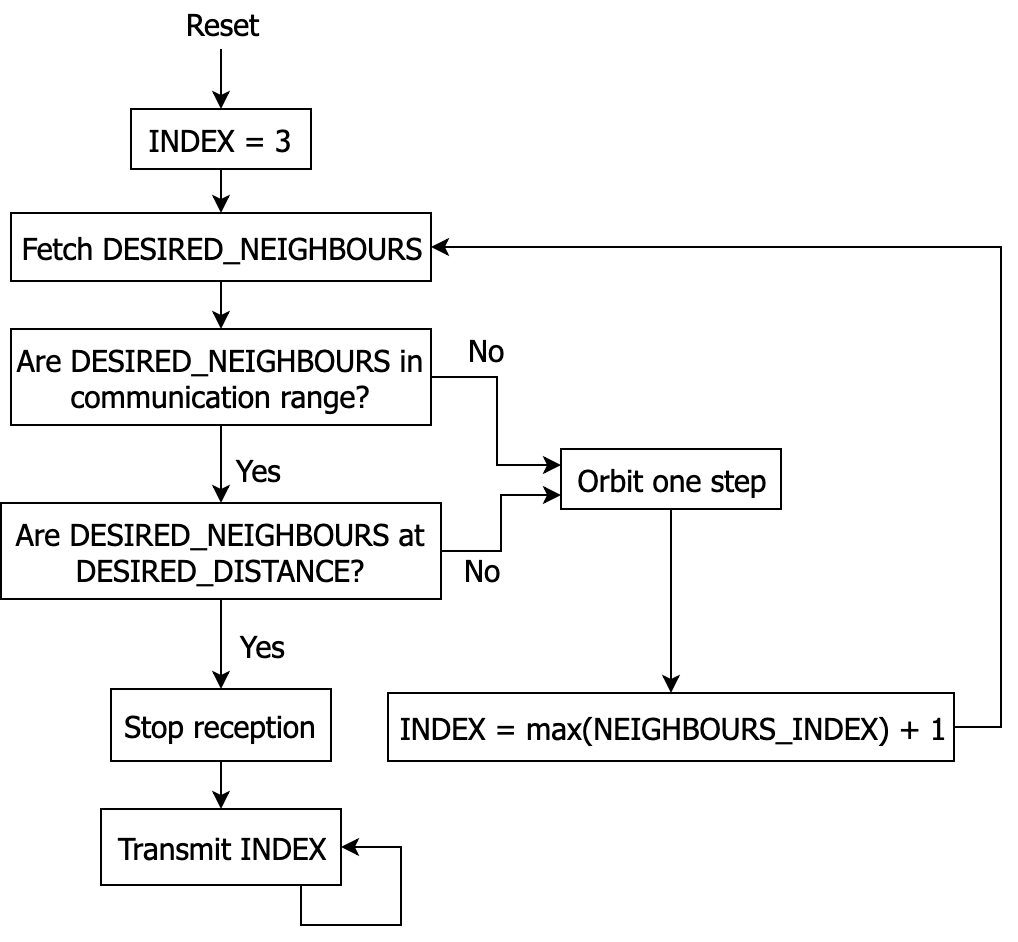
\includegraphics[scale=0.24]{shape_formation_ppt}
	\end{figure}
}
\only<4>{
	\begin{columns}[b]
		\begin{column}{0.5\textwidth}
			\begin{figure}
				\centering
				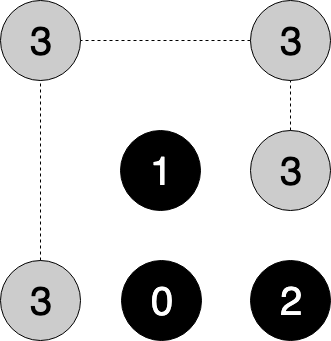
\includegraphics[scale=0.25]{shape_formation_process_1}
				\vspace{0.2cm}
				\caption{First builder}
			\end{figure}
		\end{column}
		\begin{column}{0.5\textwidth}
			\begin{figure}
				\centering
				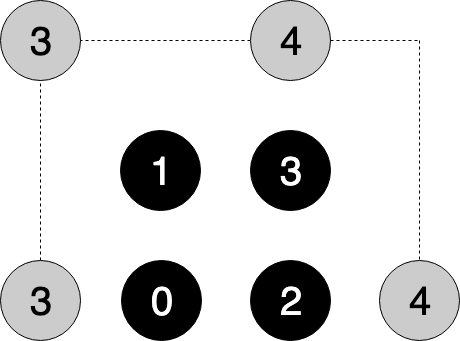
\includegraphics[scale=0.25]{shape_formation_process_2}
				\vspace{0.2cm}
				\caption{Second builder}
			\end{figure}
		\end{column}
	\end{columns}
}
\only<5>{
	\frametitle{Shape formation}
	\framesubtitle{Demonstration}
	\begin{figure}[H]
		\centering
		\fbox{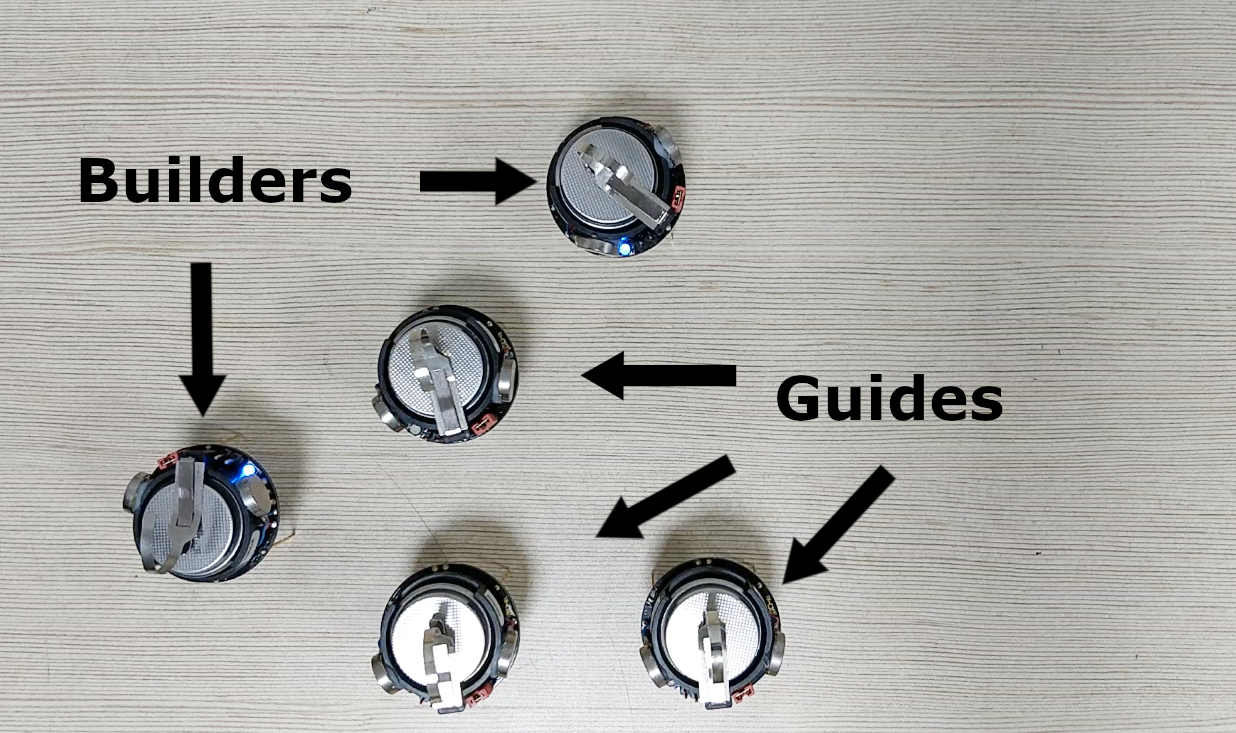
\includegraphics[width=3.5in]{shape_formation_demo}}
		\vspace{0.2cm}
		\caption{\href{https://youtu.be/SoDq9GQvNAE}{ Rectangle shape formation by Kilobots (l=3, b=2)}}
		\label{fig:shape_formation_demo}
	\end{figure}
}
\end{frame}